\section{Background and Related Works}
\label{sec_background}

\begin{figure*}[th]
	\centering
	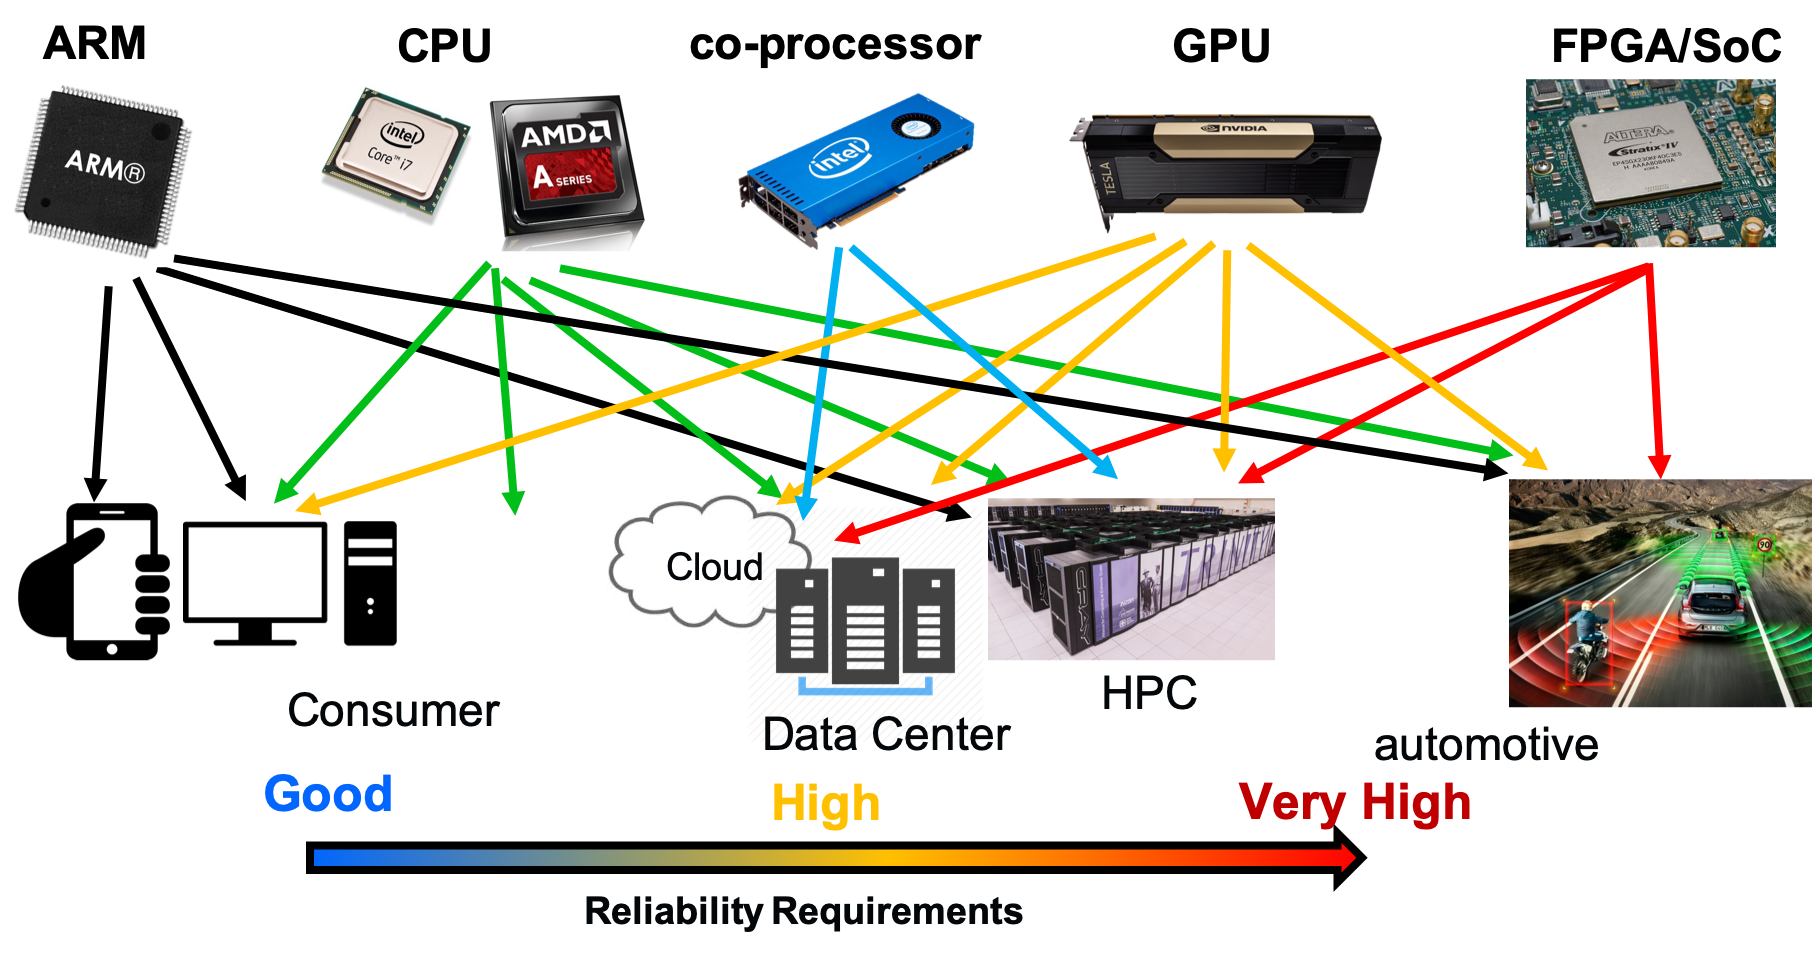
\includegraphics[width=0.75\textwidth]{./figs/motivation.png}
	\caption{High energy and thermal neutrons normalized cross sections for AMD APU and FPGA.}
	\label{motivation}
\end{figure*}

%This section serves as a background and related works on high energy and thermal neutrons effects on computing devices. 
%
%\subsection{Motivation}

Radiation is a known cause of upsets in computers~\cite{Jedec2006}. The interaction of particles, primarily neutrons for terrestrial machines, with transistors can reverse the value of the bits stored in memory or create current spikes in logic operations. These faults can create an undetected error known as Silent Data Corruption (SDC), or create a Detected Unrecoverable Error (DUE). It is well known that thermal neutrons can affect electronic devices~\cite{Baumann2005, ziegler2003}; however, only devices containing $^{10}B$ are susceptible to thermal neutrons. 
Approximately 20\% of naturally occurring Boron is $^{10}B$ with the rest primarily being $^{11}B$. Depleted Boron, where the $^{10}B$ content is low, is expensive in large quantities and generally not used in COTS parts. %Previous generations of silicon chips used borophosphosilicate glass in the manufacturing process until it was shown to increase by $8\times$ the likelihood of upsets and replaced with glass not containing boron~\cite{baumann1995boron,normand2006quantifying}. Until recently the "boron problem" was considered a solved issue, however, as our experiments show, newer silicon chips seem to have re-introduced large amounts of boron back into the manufacturing process. Understanding how this change effects overall system reliability is the primary motivation for this work.

Recently, $^{10}B$ was found in the manufacturing process of COTS devices~\cite{wen2010b10}. It is worth noting that $^{10}B$ presence does not depend on the technology node but on the quality of the manufacturing process (smaller transistors will have less Boron, but also less Silicon. The Boron/Silicon percentage is not necessarily reduced). As devices produced for the user market are now employed in HPC and safety-critical applications, we must expect $^{10}B$ to be present. 
%In fact, purified Boron is expensive and would increase the device price (unjustified for user applications). 
Some previous work has studied the sensitivity of SRAM and FPGA devices to thermal neutrons~\cite{lee2015radiation,fang2016characterization,maillard2015neutron}. Weulersse et al.~\cite{weulersse2018contribution} compared the error rates of some memories (SRAM, CLB, caches) induced by thermal neutrons, 60MeV protons, and 14MeV neutrons. %Weulersse et al. experiments were conducted on memory devices not typically used in HPC systems. In addition,many memory errors  can be masked or detected through ECC and parity on HPC systems. %Unfortunately, Weulersse et al. do not share details about the kind of errors observed during their experiments (single vs. multiple bit flips), preventing extrapolation of their results to HPC devices with ECC enabled.

%Our work advances the knowledge on HPC reliability by considering the impact of thermal neutrons  on the reliability of HPC devices.  The radiation experiments were performed on devices  executing representative applications under normal operational configurations (i.e., protection mechanisms enabled) to provide a realistic comparison between the error rates induced by high energy and thermal neutrons. Unlike previous publications, we perform both thermal and high energy neutrons experiments on exactly the same devices in the same conditions to limit comparison uncertainty. Furthermore, for the first time, we investigate through thermal neutron detector measurements, how modern data center construction and cooling systems designs influence the thermal neutron flux and the HPC system fault rates.

\subsection{High Energy and Thermal Neutrons}
\label{sec_environment}

\textbf{High energy} neutrons, or fast neutrons, are neutrons with energies that range from 1 to over 1,000 MeV are known to disturb the function of electronic devices and are considered a main cause of faults in terrestrial electronic devices~\cite{Baumann2005,ziegler2004ser}. %High energy neutrons primarily interact with silicon chips via elastic scattering which can deposit thousands of electron-Volts (eV, a standard unit of energy used in nuclear physics) of energy into a recoil nuclei. 
%Neutron scattering may also produced secondary particles such as protons or alphas. All of these processes can free bound electrons in large enough quantities to alter the behavior of the circuits on a chip which may induce faulty behavior in one or more bits. Permanent damage can also occur due to the displacement of atoms within a chip.
The flux of high energy neutrons in the atmosphere has been thoroughly studied since Hess' discovery~\cite{Hess,Ziegler1996}. The flux is known to vary across the surface, as a consequence of the earth's magnetic field, and increases exponentially with altitude, reaching a maximum at about 60,000 ft. Under normal solar conditions, the fast neutron flux is almost constant for a given latitude, longitude, and altitude. 

\textbf{Thermal} neutrons, or slow neutrons, are low energy neutrons (lower than 0.5 eV), produced by the moderation of high energy neutrons in materials or the emission of neutrons from nuclear decay. 
%Incident high energy neutrons rain down as part of cosmic ray induced showers reaching thermal energies after 10-20 interactions. %Thermal neutrons continue moving until they are either absorbed in a nuclear reaction, or decay (whilst stable in atomic nuclei, free neutrons have a half-life of about 10 minutes).
%When a thermal neutron is absorbed by $^{10}B$,  the resulting isotope decays, producing a Lithium isotope and an alpha particle. Both the Lithium isotope and alpha particle can induce faults. The amount of boron in a particular computing device is proprietary information that is not disclosed by industry. The only definitive way to evaluate the thermal neutron sensitivity of a device is to expose it to thermal neutrons. 
%
The flux of thermal neutrons, in contrast to high energy neutrons, can be difficult to predict as it strongly depends on the environmental conditions as well the presence of other materials (primarily hydrogen containing) in the device's immediate surroundings (like concrete, water, a fuel tank, etc..) in addition to latitude, longitude, and altitude. Various authors have made calculations to evaluate thermal fluxes in realistic cases~\cite{ziegler2003, hands2011single, baumannsoft, sheu2003cosmic}. As a result, when predicting the error rate caused by thermal neutrons, it is essential to measure rates in realistic settings. 

We have built and deployed a neutron detector in order to have a precise understanding of the thermal neutron flux inside a representative data center. We measured the rates of thermal neutrons in the proximity of water, and demonstrate that cooling water, for instance, can increase the thermal neutron flux (and thus error rate) by up to 20\%. %In Section~\ref{sec_fit} we estimate the high energy vs. thermal neutrons error rate for two locations with known neutron fluxes and discuss the effects of environmental conditions (sunny and rainy day) and surrounding materials (concrete slab floors).


\subsection{Supercomputer Cooling}
\label{sec_cooling}

One of the main challenges in designing HPC systems is the dissipation of heat. A modern supercomputer can push more than 750 watts per square foot which can easily overwhelm traditional cooling systems~\cite{patterson2008state}.
%The power and heat density in a single rack of current supercomputers demands
%efficient and reliable cooling techniques to keep the components at
%operational temperatures.
%Today's supercomputers consist of hundreds of computing racks (e.g., Summit uses 256 racks~\cite{summit-overview}), requiring specific room
%designs to optimize both cooling efficiency and ease of maintenance. 
%Hot/cold air segregation and raised floors are the most common design strategies 
%for new supercomputers~\cite{patterson2008state}.
%
%Air segregation for hot and cold air aisles may require nonstructural walls
%added to the building to make the physical segregation of the aisles. These
%additional walls and the structural ones, as demonstrated in
%Section~\ref{sec_fit}, act as a moderator for neutrons energy and, thus,
%increase the thermal neutron flux. Similarly, raised floors, designed to
%increase the flexibility for routing liquids, power and network, may also
%collaborate to increase the thermal neutron flux as their structure requires
%additional concrete.
%
One notable and growing trend in data centers is the use of 
liquid cooling~\cite{capozzoli2015cooling}. Eight of today's Top10
supercomputers use some form of liquid cooling~\cite{Dongarra2013}. 
These surrounding materials, as demonstrated in Section~\ref{sec_fit}, act as a moderator for neutrons energy and, thus, increase the thermal neutron flux.
%Liquid cooling is more efficient at heat removal than traditional air cooling and using it 
%allows for an overall increase in performance and power efficiency.
%Traditional data
%centers may use 25\% to 35\% of their energy budget just for cooling. IBM
%chiller-less water cooling systems have been shown to reduce the cooling energy
%overhead to just 3.5\%~\cite{gao2015experimental}. IBM has noted that using liquid 
%cooling in can allow for a 34\% increase in processor frequency which can increase system performance by approximately
% 33\% ~\cite{ellsworth2008evolution,ellsworth2012overview}. 

\subsection{Motivation}
\label{sec_mot}

As mentioned, it is mainly the presence of $^{10}B$ in the manufacturing process that makes a device susceptible to thermal neutrons~\cite{wen2010b10}. Reducing the amount of $^{10}B$ could reduce the sensitivity of the device to thermal neutrons accordingly and using purified Boron would make the device immune to thermal neutrons induced effect.

Nevertheless, the use of purified Boron increases the manufacturing process and, thus, the final product cost. Such an increased cost is unjustified for consumer electronics, as the (high energy or thermal) neutrons error rate is sufficiently low not to be considered a major concern for user applications (video editing, gaming, and so forth). Having a more expensive product to ensure high reliability is not appealing for the consumer and manufacturers are investing in improving performances and efficiency as well as in improving the yield. 

Lately, applications for which reliability is indeed a major concern, as cloud computing, High Performance Computing, and automotive applications, have started to be powered by COTS devices. The choice of using COTS in these applications is dictated by the need of extremely high computational requirements with low power budget. The automotive market is a corner case. To implement an autonomous vehicle it is necessary to detect objects in real time, and this is normally achieved though Convolutional Neural Networks (CNNs) that are very computational demanding. Moreover, high computational efficiency is preferred in order not to exceed the vehicle power budget. Finally, the manufacturing cost is a highly sensible variable as the automotive market is highly competitive. As a result, the device selected to execute CNNs for autonomous vehicle must be efficient, with high performances, and low-cost as a COTS device. Nevertheless, reliability must be paramount, and this must include the thermal neutron component.

Figure~\ref{motivation} shows an abstract view of the current COTS devices market situation. There are various computing architectures available in the market, from low power ARM embedded processors to high end CPU, accelerators as co-processors or GPUs, and programmable or application-specific devices (FPGAs or ASICs). Each of these devices has its own computing characteristics and cost. Most producers are willing to increase the yield by adopting the same architecture for various application domains, from consumer electronic, to cloud serves, HPC, and autonomous vehicles. Nevertheless, the strategy works only if the COTS device reliability is carefully evaluated and found to be sufficient for the project requirements. 

$^{10}B$, which is the main topic of this paper, is one of the main variables in the reliability evaluation of COTS devices. As said, manufacturers do not have interest in using the more expensive purified Boron for their devices as this could put them in a weaker market position and reduce their yield. On the other hand, when the COTS device is employed as part of a project that has high reliability requirements it is mandatory to evaluate also its thermal neutrons induced error rate. We cannot assume that a device that was not produced to be highly reliable is $^{10}B$ free.

As mentioned, the second very important aspect of thermal neutrons reliability evaluation, besides the presence of $^{10}B$ and the device sensitivity to thermal neutrons, is the thermal neutron flux. While the high-energy neutrons flux has been extensively studied and is assumed to be relatively constant (but dependent on the location), the thermal neutrons flux is extremely variable. Humidity, location, materials in proximity of the computing device (such as water, wood, concrete, gasoline, and so forth) are among the several factors that can significantly modify the thermal neuron flux and, then, the final FIT rate of the COTS device. As an example, when it rains the error rate of a device detecting objects in a car can be significantly higher than during a sunny day, in a supercomputer devices placed close to the water-cooling pipes can experience a higher fault rate than other nodes. It is the goal of this paper to understand also the variability of the error rate of devices based on some of these variables.



